\documentclass[11pt]{article}
\usepackage{preprint}
\captionsetup[figure]{name=Fig.,labelsep=period}

\title{Lessons from Post-Katrina Expansion of Charter Schools in New Orleans}
\author{Jiadi He\email{jh2288@georgetown.edu}}
\affil{Georgetown University}
\shorttitle{Post-Katrina Charter Schools in New Orleans}
\keywords{school governance; markets; accountability}

\begin{document}
\maketitle
\keywordsline

In the wake of the devastating tragedy that befell New Orleans after Hurricane Katrina in 2005, the government used the chance to carry out a controversial experiment-replacing public school with charter schools. The move was almost unthinkable because it sought to replace traditional education schools with charter schools that would be operated by private entities but funded by the public. Hurricane Katrina destroyed 100 out of the 128 public school buildings in New Orleans (Alzahrani, 2018). The decision to replace public schools with charter schools may have been a solution to the immediate challenge. However, it also portrayed a challenge with the education system in New Orleans and the need to change how public schools operated. Handing over public schools to a private charter means that schools would not be controlled by the government as before. The newly found freedom led to a change in curricula, teacher unions, attendance zones, and a change in many basic regulations. As explained in the current analysis, this change was an effective chance for public school officials, charter school officials, and public officials to learn. The analysis is banked on the thesis that school management systems are critical to students’ performance, therefore, schools should ensure they use the most effective approaches.

The first lesson change in the reformed system was that after the state handed over the management of schools to the non-profit charter, the charter implemented strict requirements for the key stakeholders like teachers to follow. The level of accountability increased and teachers were hired on performance-based contracts. The new school leaders were given authority to manage all teaching and non-teaching staff, and parents would choose the schools where their children attended (Harris, 2020). The outcomes of this new management style were that performance improved and school attendance increased. According to Harris (2020), this improvement emanated from a combination of government and private control. Thus, although the private charter triggered this improvement, the government played a critical role in ensuring the successful implementation of the programs. Thus, the explicit first lesson to the public school officials, charter school officials, and public officials was that market pressures are good but work best when the government is involved. The implicit lesson was that although it is tempting to dismiss the effectiveness of the traditional school system used in New Orleans before Hurricane Katrina, this system was effective in ensuring students' success.

The second lesson was that the traditional school system was unfit for New Orleans because it gave too much freedom to school management, which led to poor management. The reforms changed the status quo that had allowed the oppression of African Americans for many years. According to Harris (2020), the reforms allowed families to choose the school of their choice from a list of charter schools. The freedom to choose made it possible for parents to find schools they found suitable for their children. The new system also added pressure on schools to perform because this performance would determine the likelihood of becoming the choice for many students. After the reshuffled management in New Orleans, students’ scores changed as shown below:

\begin{figure}[!htbp]
\centering
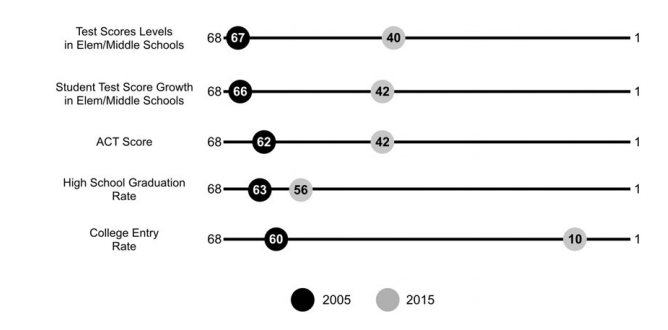
\includegraphics[width=0.85\linewidth]{figure1.png}
\caption{New Orleans’s statewide rankings on student outcomes in 2005 (black circles) and 2015 (gray), before and after the reforms (based on a total of 68 districts) (Harris, 2020)}
\label{fig:rankings}
\end{figure}

The figure implies a significant improvement in scores after the change in management. The author gives specific improvements as follows: test scores increased from 35\% to 62\%, ACT scores rose from 17 to 18.4 points, high school graduation from 54\% to 73\%, and college entry from 37\% to 63\% (Harris, 2020). When evaluating the possible reasons for the improved performance after the reforms, Harris points out that one of the possible drivers of the improved performance is attributed to the autonomy that schools gained to hire and fire teachers. The others were the high competition for students and resources by schools and the power of the government to shutter, takeover, or transfer school management in low-performing schools. The fact that school management could be fired or transferred by the government made school heads and teachers more committed to their work. The implicit lesson was that school heads and teachers in government-managed schools are reluctant and negligent due to lack of close monitoring.

The other lesson is that schools are part of a market system affected by demand, supply, and customer satisfaction. In the reformed structure, the government would take punitive steps on teachers found to underperform by transferring them or firing them. The rationale behind the decisions would represent customer satisfaction. The flexibility of choosing schools by parents represented demand and supply trends based on customer satisfaction. Competition for best-performing schools led to a market system where teachers and other stakeholders had to earn their ratings. This finding implied that, just like businesses, education was prone to market forces. According to Harris (2020), the interplay between the government and markets was behind the improved results. Overall, this relationship achieved high performance.

The last lesson is that inequities affect schools’ performance. According to Vergari (2007), one of the reasons why the post-Katrina educational reforms in New Orleans attracted public attention because it challenged the legitimacy of the traditional funding and management in public schools. Vergari also acknowledges that the reforms in New Orleans exposed the inequalities that the traditional system created in the education system. The fact that charter schools received less funding because they predominantly served minority groups showed the racial discrimination in the education system and its implications on education. According to Harris (2020), the reforms led to a shift in the racial composition of the teachers from three-quarters Black to majority white and reduced the democratic voting rights that stakeholders had on the running of their schools. The outcomes from this change show that it benefited learners and improved school management. This improvement teaches public school officials that racial segregation and other inequalities harm education. This paper focuses on the positive implications of the changes and its findings are generalizable because they are based on facts that relate to most schools. The stakeholders, including charter and public school officials, policy makers, and legislators, draw the same lessons from this case study because the causes and effects are similar. All factors involved in the case can be interpreted the same by all of them.

Conclusively, the post-Katrina educational reforms in New Orleans show improvements that act as lessons to public school officials, charter school officials, and public officials regarding the management approach they use, their impacts, and ways of improving it. As explained in the current analysis, the reforms portrayed the failures of the traditional education system and how they led to educational failures in New Orleans. The reforms also indicate that charter schools are more effective when they work with the government.

\begin{references}
\item Alzahrani, S. (2018). New Orleans Educational System in Public Schools Pre/Post Hurricane Katrina as Perceived by Special Education Teachers. \textit{World Journal of Education}, \textit{8}(2), 88-94.
\item Harris, D. N. (2020). \textit{Charter school city: What the end of traditional public schools in New Orleans Means for American education}. University of Chicago Press.
\item Vergari, S. (2007). The politics of charter schools. \textit{Educational Policy}, \textit{21}(1), 15-39.
\end{references}

\end{document}
